\documentclass[tikz]{standalone}
\usetikzlibrary{decorations.pathreplacing,calc,automata,arrows}
\begin{document}

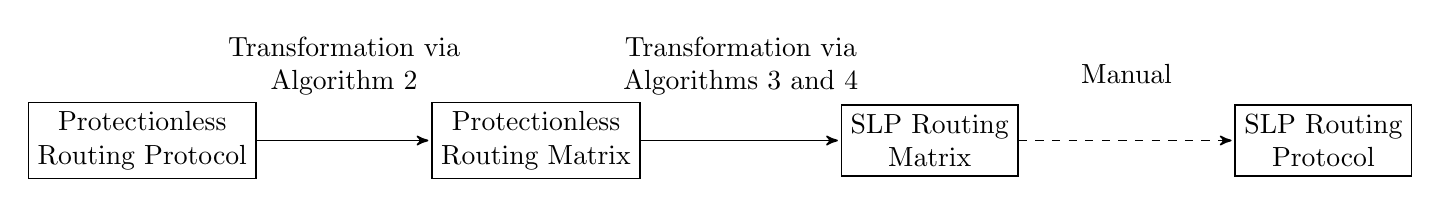
\begin{tikzpicture}[->,>=stealth',shorten >=1pt,semithick]
\begin{scope}[auto, every node/.style={minimum size=2.2em}]

\node[draw,align=center] (p1) at (-5,0) {Protectionless\\Routing Protocol};
\node[draw,align=center] (p2) at (0,0) {Protectionless\\Routing Matrix};
\node[draw,align=center] (p3) at (5,0) {SLP Routing\\Matrix};
\node[draw,align=center] (p4) at (10,0) {SLP Routing\\Protocol};

\draw [->] (p1) to node[text width=6cm,align=center,shift={(0,3ex)}]{Transformation via\\Algorithm 2} (p2);
\draw [->] (p2) to node[text width=3cm,align=center,shift={(0,3ex)}]{Transformation via\\Algorithms 3 and 4} (p3);
\draw [->,dashed] (p3) to node[text width=3cm,align=center,shift={(0,3ex)}]{Manual} (p4);

\end{scope}
\end{tikzpicture}

\end{document}
